\documentclass[11pt,a4paper]{article}
\usepackage{fontspec}
\setmainfont{TeX Gyre Pagella}
\newfontfamily\headfont{Inter}[UprightFont=*-ExtraBold,BoldFont=*-ExtraBold,Extension=.otf,Path=/usr/share/fonts/opentype/inter/]
\usepackage[a4paper,margin=2.3cm]{geometry}
\usepackage{graphicx,booktabs,float,caption,array,xcolor,longtable}
\usepackage{xurl}
\usepackage[hidelinks]{hyperref}
\usepackage{titlesec}
\usepackage[round]{natbib}
\usepackage{setspace}
\setstretch{1.05}
\renewcommand{\topfraction}{0.9}
\renewcommand{\bottomfraction}{0.8}
\renewcommand{\textfraction}{0.1}
\renewcommand{\floatpagefraction}{0.75}
\setlength{\parindent}{0pt}
\setlength{\parskip}{0.55em}
\titleformat{\section}{\headfont\Large}{\thesection}{0.8em}{}
\titleformat{\subsection}{\headfont\large}{\thesubsection}{0.8em}{}
\captionsetup{font=small,labelfont=bf}
\urlstyle{same}
\hypersetup{pdftitle={Every Tsunami on Record},pdfauthor={Tristan Hotham}}

\begin{document}
\begin{center}
{\Large\bfseries Every Tsunami on Record\par}
\vspace{0.4em}
{\large Sources, runups and deaths in NOAA's Global Historical Tsunami Database,\\1610 BC to 2026\par}
\vspace{1.2em}
{\large Tristan Hotham\par}
\vspace{0.3em}
{\small Independent researcher\\
ORCID: 0000-0003-4931-9349\\
DOI: https://doi.org/10.5281/zenodo.23873531\par}
\vspace{0.8em}
2026
\end{center}

\begin{quote}
\small
\begin{center}\textbf{Abstract}\end{center}
I map and describe every tsunami that NOAA's National Centers for Environmental Information (NCEI) rate as definite or probable in the Global Historical Tsunami Database: 1,699 source events from 1610 BC to 2026, with 33,532 records of the places their water reached. 72\% were started by an earthquake alone and 79\% involved an earthquake; 63\% of earthquake sources lie within 100 km of a plate boundary. 67\% began in NCEI's Pacific regions and 67\% on the Pacific rim, the Ring of Fire. NCEI records 545,939 tsunami deaths for 244 events; the Indian Ocean tsunami of 2004 accounts for 42\% and the ten deadliest for 78\%, while the Indian Ocean as a whole has 5.8\% of tsunamis but 50\% of deaths. The highest runups come not from great ocean tsunamis but from landslides into narrow bays, led by 524.3 m at Lituya Bay, Alaska, in 1958: all 9 tsunamis with a runup of 100 m or more involved a landslide or a volcano. Ocean-crossing waves arrive on a timetable, at a median 680 km an hour beyond 1,000 km, close to the shallow water speed over a deep ocean; the farthest measurement is 19,266 km from Sumatra in 2004. The number of tsunamis recorded per century rises from 63 in the 1600s to 718 in the 1900s, a measure of recording, not of hazard.

\textbf{Keywords:} tsunamis; natural hazards; earthquakes; landslides; volcanoes; runup; disaster mortality; NOAA NCEI; open data; mapping
\end{quote}

\section{Introduction}
A tsunami is a train of long waves set off when a large volume of water is displaced at once, most often by the sudden movement of the sea floor in an earthquake, but also by landslides, volcanic eruptions and collapses, explosions and fast moving atmospheric disturbances. Near the source a tsunami can run tens or even hundreds of metres up the shore; far away it may register as a few centimetres on a tide gauge. NCEI and the World Data Service maintain the Global Historical Tsunami Database \citep{ncei}, which brings together historical accounts, geological evidence, tide gauge and deep-ocean records and post-tsunami surveys for every event they can document. This paper takes the whole database as it stood in 2026 and asks simple questions of it: where tsunamis start and why, where their water was recorded, how high it ran, how far and how fast it travelled, and how many people died. An interactive map accompanies the paper at \url{https://maps.tristanhotham.com/tsunamis/}.

\section{Data and methods}
\subsection{Source events}
The database was fetched from the NCEI Hazard Service API (\url{https://www.ngdc.noaa.gov/hazel/hazard-service/api/v1/}), endpoints \texttt{tsunamis/events} and \texttt{tsunamis/runups}. It holds 3,138 source events. NCEI rates each event's validity as 4 (definite tsunami), 3 (probable), 2 (questionable), 1 (very doubtful), 0 (an event that only caused a seiche or a disturbance in an inland river or lake) or $-1$ (an erroneous entry). I count only events rated 3 or 4: 1,699 tsunamis (1,110 definite and 589 probable), leaving out 1,439 entries. Of the 1,699, 1,583 have a position.

NCEI's cause codes are: 0 unknown, 1 earthquake, 2 questionable earthquake, 3 earthquake and landslide, 4 volcano and earthquake, 5 volcano, earthquake and landslide, 6 volcano, 7 volcano and landslide, 8 landslide, 9 meteorological, 10 explosion and 11 astronomical tide. I checked these against the data before use: the Halifax munitions explosion of 1917 carries code 10; the Vajont dam landslide of 1963, the Lituya Bay rockslide of 1936 and the Dickson Fjord rockslide of 2023 code 8; Krakatau in 1883 and Hunga Tonga in 2022 code 6; codes 4 to 7 almost always carry a linked volcano record and codes 1, 3 and 8 almost never; and code 9 events have no earthquake magnitude and include a run of meteotsunamis in south-western Australia. I group the codes into earthquake (1 and 2), earthquake and landslide (3), volcano (4 to 7), landslide (8), meteorological (9), explosion (10) and unknown (0 and 11). Table~\ref{tab:causes} gives the counts by code.

\begin{table}[tbp]\centering\small\caption{Definite and probable tsunamis by NCEI cause code, and the groups used here.}\label{tab:causes}\begin{tabular}{rllr}\toprule Code & NCEI cause & Group & Tsunamis\\\midrule
0 & Unknown & Unknown & 48\\
1 & Earthquake & Earthquake & 1,219\\
2 & Questionable earthquake & Earthquake & 5\\
3 & Earthquake and landslide & Earthquake and landslide & 115\\
4 & Volcano and earthquake & Volcano & 8\\
5 & Volcano, earthquake and landslide & Volcano & 2\\
6 & Volcano & Volcano & 74\\
7 & Volcano and landslide & Volcano & 19\\
8 & Landslide & Landslide & 131\\
9 & Meteorological & Meteorological & 76\\
10 & Explosion & Explosion & 2\\
11 & Astronomical tide & Unknown & 0\\
\midrule & All & & 1,699\\\bottomrule\end{tabular}\end{table}

Each event carries an NCEI region code. I group these into oceans (Pacific, regions 80 to 89; Indian Ocean, 60; Atlantic and Caribbean, 70 to 77; Mediterranean, 50; Black Sea and Caspian, 40; Red Sea and Persian Gulf, 30; inland Africa, 78), and treat regions 81 to 89, the rim of the Pacific without Hawaii, as the Ring of Fire. One event has no region. For earthquake sources I measured the great-circle distance to the nearest boundary in Bird's PB2002 plate model \citep{bird}.

\subsection{Deaths}
NCEI gives two death figures: the deaths caused by the tsunami, and the total for the whole event including the earthquake, eruption or landslide that caused it. The two can differ enormously. I use only the first. For many events, especially old ones, NCEI gives no figure or only an order of magnitude (73 tsunamis), so totals are a floor.

\subsection{Runups and travel}
The 35,129 runup records are places where the water was recorded: survey marks, tide gauges, eyewitness accounts and deep-ocean pressure gauges. I keep the 33,532 that belong to a definite or probable tsunami and are not flagged doubtful (1,248 are). NCEI's doubtful field also uses two other flags, which I checked against the data: one marks places where the water moved with the atmospheric pressure wave of a great eruption (727 records, all for Hunga Tonga and Krakatau) and one marks meteorological sources. I keep both, but leave the air wave places out of the distance and speed results. The 356 deep-ocean gauge records are left out of the map, the country counts and the distance results. Height is NCEI's maximum water height at the place, distance its great-circle distance from the source, and travel time its hours and minutes from the event to the first arrival. Death figures attached to runup places are not summed, because a town and its prefecture can both appear.

\section{Results}
\subsection{How many, and what starts them}
Figure~\ref{fig:map} maps every source and every place. 1,224 tsunamis (72.0\%) were started by an earthquake alone, 115 (6.8\%) by an earthquake with a landslide, 131 (7.7\%) by a landslide, 103 (6.1\%) by volcanic activity, 76 (4.5\%) by meteorological disturbances and 2 by explosions; 48 have no known cause (Figure~\ref{fig:causes}). Among the 1,219 earthquake sources with a magnitude, the median is 7.1, 63\% are 7 or more and 7 are 9 or more. 62.6\% of earthquake sources with a position lie within 100 km of a PB2002 plate boundary and 91.7\% within 250 km (median 74 km). Volcanoes cause 6.1\% of tsunamis but 9.8\% of recorded deaths.

\begin{figure}[tbp]\centering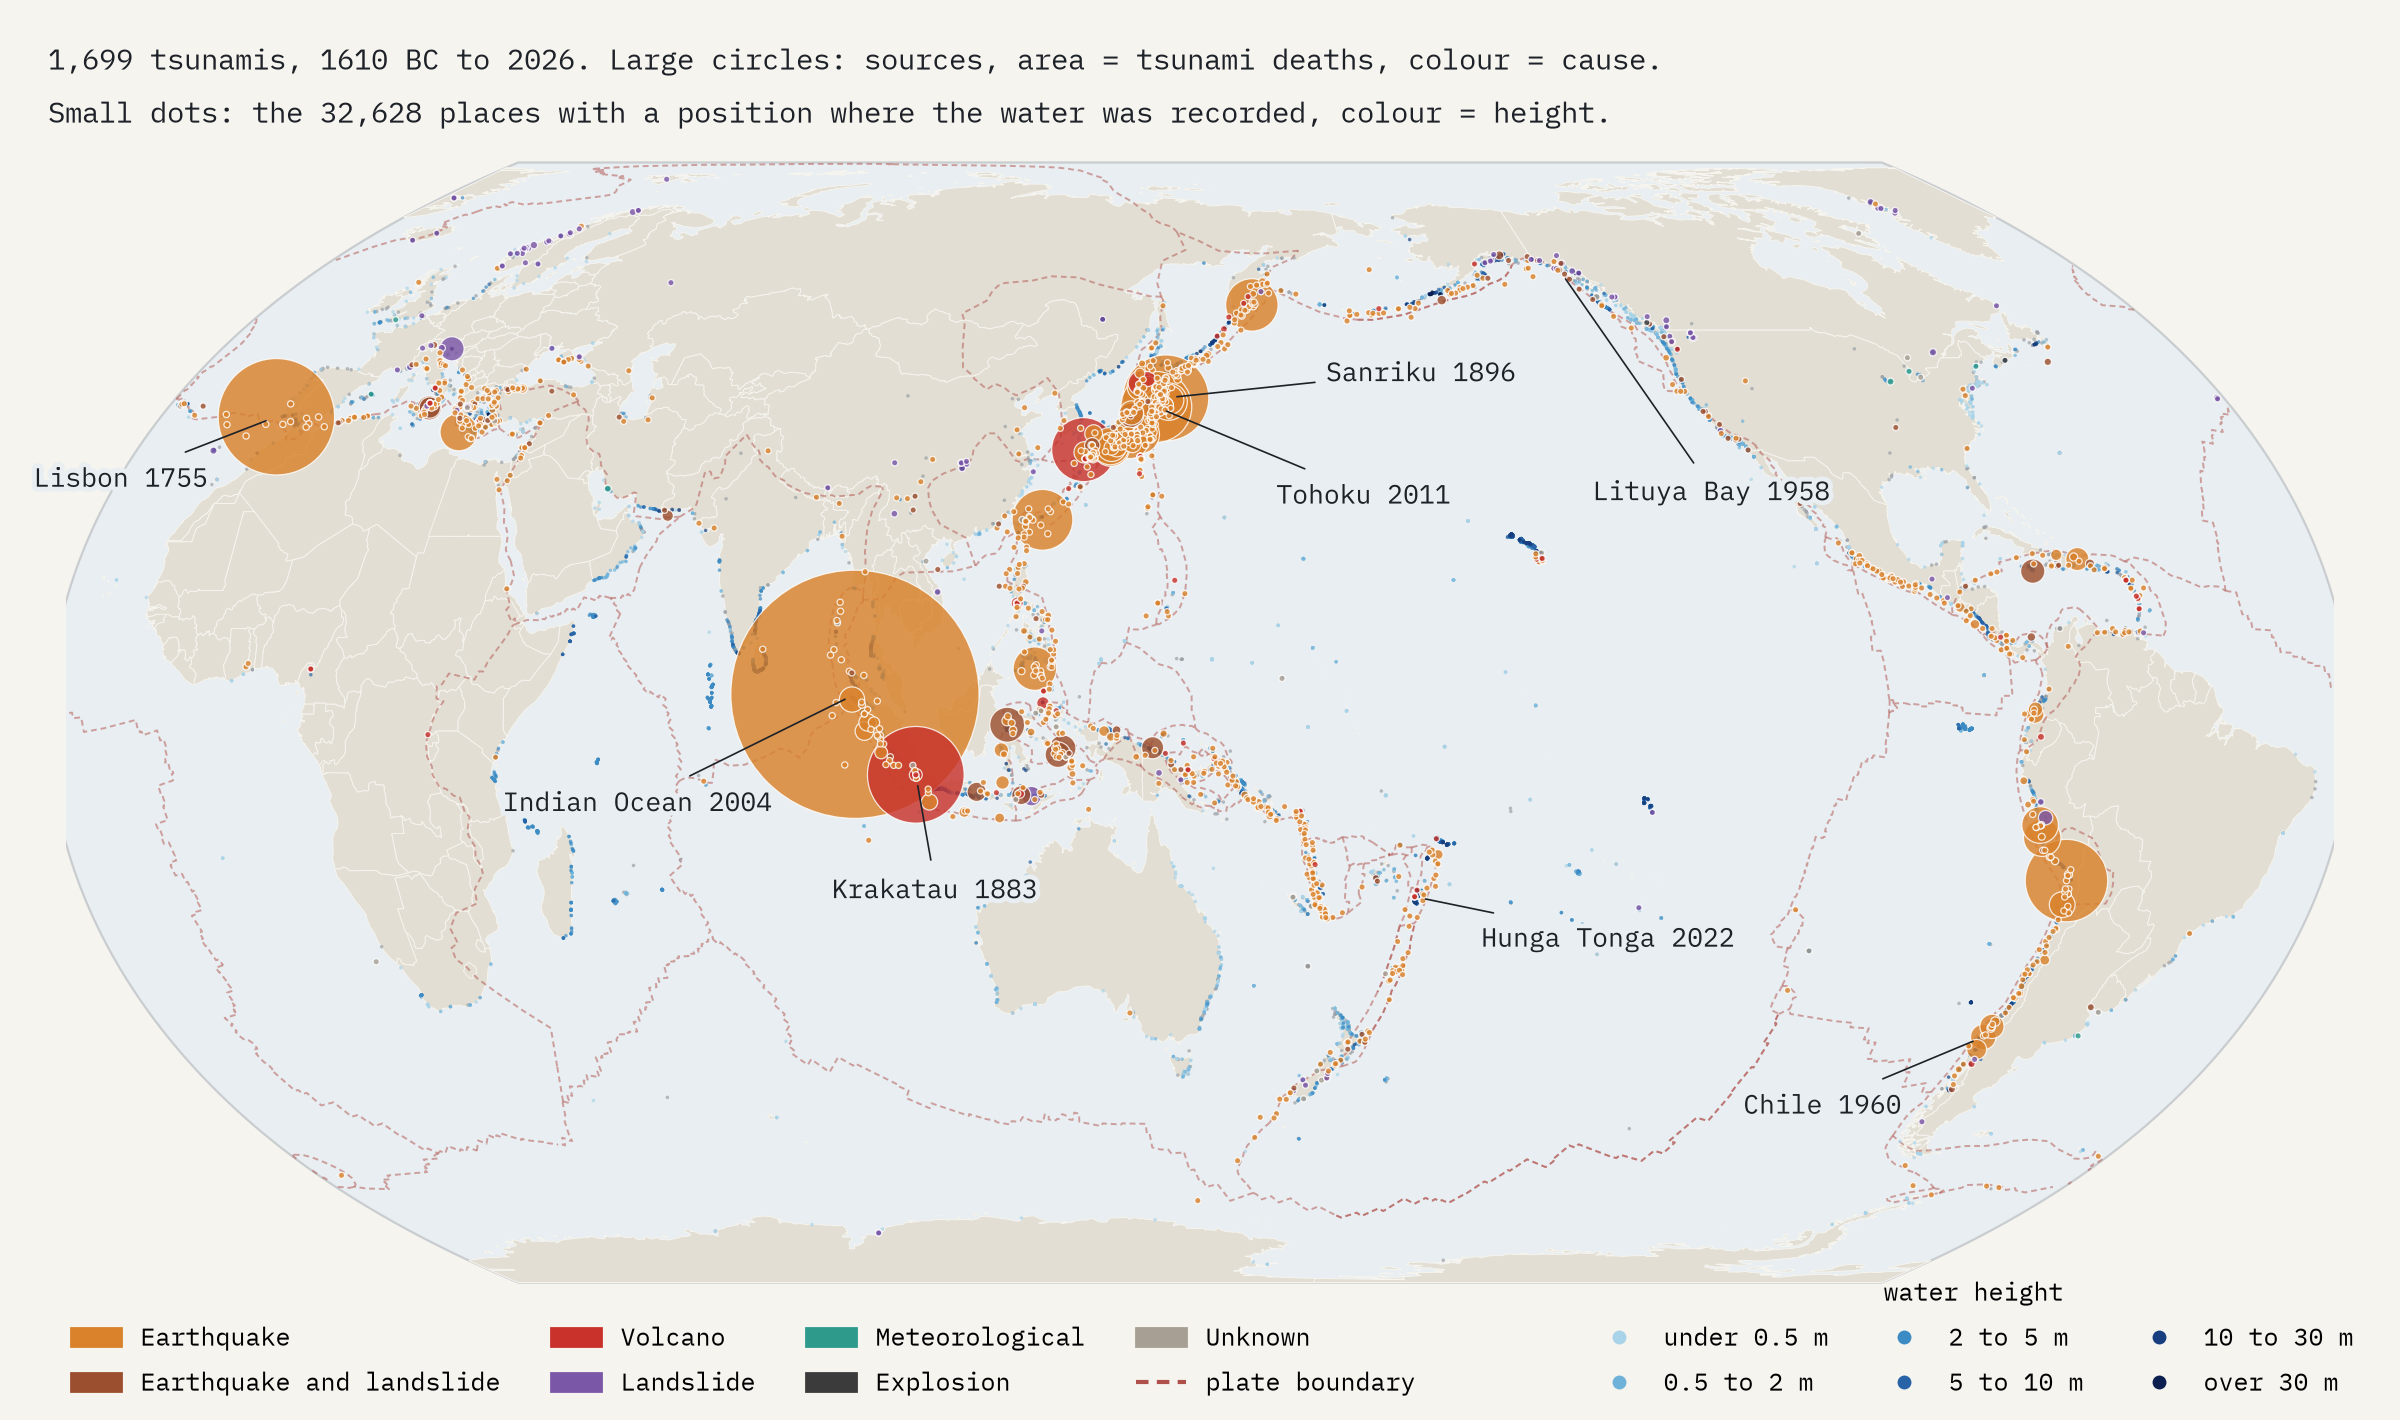
\includegraphics[width=\textwidth]{f_map.png}
\caption{Every definite or probable tsunami source with a position, sized by tsunami deaths and coloured by cause, with the places where the water was recorded coloured by height. Pacific-centred Equal Earth projection; dashed lines: PB2002 plate boundaries.}\label{fig:map}\end{figure}

\begin{figure}[tbp]\centering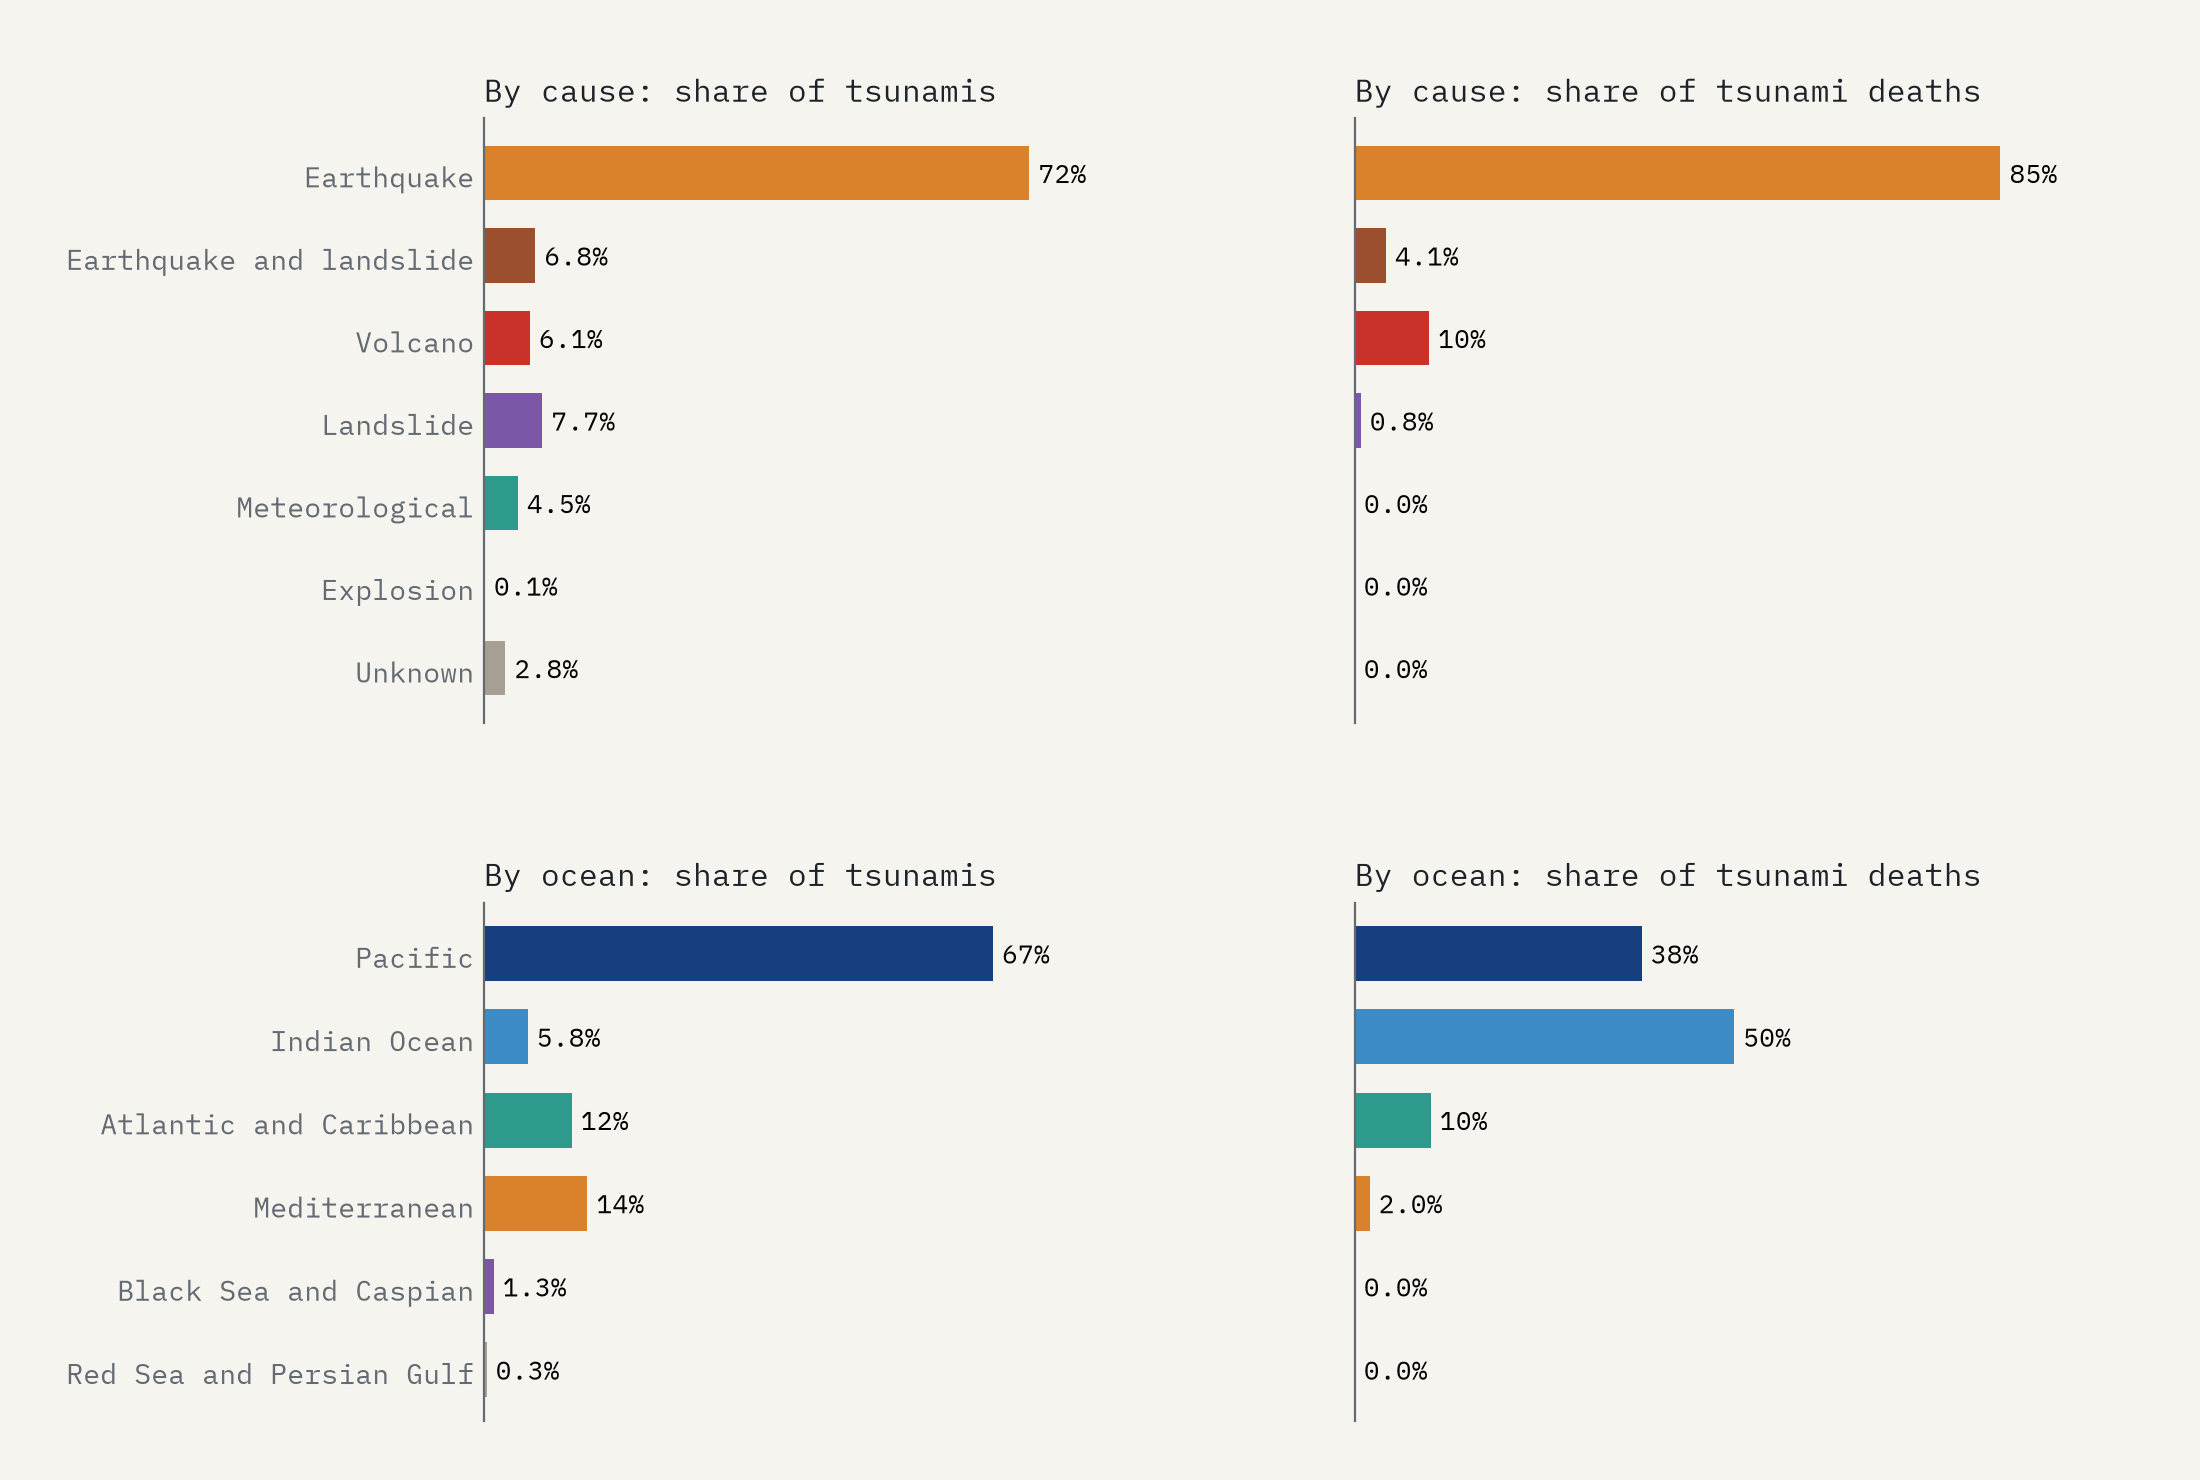
\includegraphics[width=.92\textwidth]{f_causes.png}
\caption{Share of tsunamis and of recorded tsunami deaths by cause group and by ocean.}\label{fig:causes}\end{figure}

\subsection{Where}
1,142 tsunamis (67.2\%) began in NCEI's Pacific regions and 1,131 (66.6\%) on the Pacific rim; adding the 63 tsunamis off Sumatra and Java, on the Sunda arc that NCEI places in the Indian Ocean, would raise the share to 70.3\%. Japan alone has 304 (17.9\%). The Mediterranean has 232 (13.7\%), the Atlantic and Caribbean 197 (11.6\%) and the Indian Ocean 98 (5.8\%). Deaths are distributed very differently: the Indian Ocean has 50.1\% of recorded tsunami deaths, the Pacific 37.9\% and the Atlantic and Caribbean, mostly Lisbon in 1755, 10.0\%.

Counting places where water was recorded, 140 countries and territories have been reached by at least one tsunami. Japan has been reached by 395 different tsunamis, the United States by 264 and Indonesia by 138 (Figure~\ref{fig:countries}). Japan also has 38.4\% of all place records, 6,326 of them from the surveys after the Tohoku tsunami of 2011.

\subsection{Deaths}
NCEI records tsunami deaths for 244 tsunamis (14.4\%), totalling 545,939 (Table~\ref{tab:deaths}, Figure~\ref{fig:deadliest}). The Indian Ocean tsunami of 26 December 2004 accounts for 227,899 (41.7\%), and the ten deadliest for 78.4\%. 51 tsunamis killed 1,000 people or more and 9 killed 10,000 or more. 54.4\% of recorded deaths are from 1900 or later and 46.3\% from 2000 or later, a reflection both of the 2004 disaster and of better counting. The whole-event figure tells a different story: its largest entry is the Haiti earthquake of 2010 (316,000 deaths, of which NCEI attributes 7 to the tsunami), followed by 2004 and the Great Kanto earthquake of 1923 (105,385, tsunami 325).

\begin{table}[tbp]\centering\footnotesize\setlength{\tabcolsep}{4pt}\caption{The twelve deadliest tsunamis: NCEI's tsunami deaths and its total for the whole event (including the earthquake or eruption).}\label{tab:deaths}\begin{tabular}{lllllrr}\toprule Source & Year & Country & Cause & Mag. & Tsunami deaths & Whole event\\\midrule
Off W. Coast of Sumatra & 2004 & Indonesia & Earthquake & 9.1 & 227,899 & 227,899\\
Lisbon & 1755 & Portugal & Earthquake & 8.5 & 50,000 & 50,000\\
Krakatau & 1883 & Indonesia & Volcano &  & 34,417 & 36,417\\
Sanriku & 1896 & Japan & Earthquake & 8.3 & 27,122 & 27,122\\
Northern Chile & 1868 & Chile & Earthquake & 8.5 & 25,000 & 25,000\\
Honshu Island & 2011 & Japan & Earthquake & 9.1 & 18,423 & 18,423\\
Shimabara Bay, Kyushu Island & 1792 & Japan & Volcano & 6.4 & 15,000 & 15,000\\
Ryukyu Islands & 1771 & Japan & Earthquake & 7.4 & 13,486 & 13,486\\
Kamchatka & 1952 & Russia & Earthquake & 9 & 10,000 & 10,000\\
Moro Gulf & 1976 & Philippines & Earthquake & 8 & 6,800 & 8,000\\
Off SW Boso Peninsula & 1703 & Japan & Earthquake & 8.2 & 5,233 & 5,233\\
Crete & AD 365 & Greece & Earthquake & 8 & 5,000 & 5,000\\
\bottomrule\end{tabular}\end{table}

\begin{figure}[tbp]\centering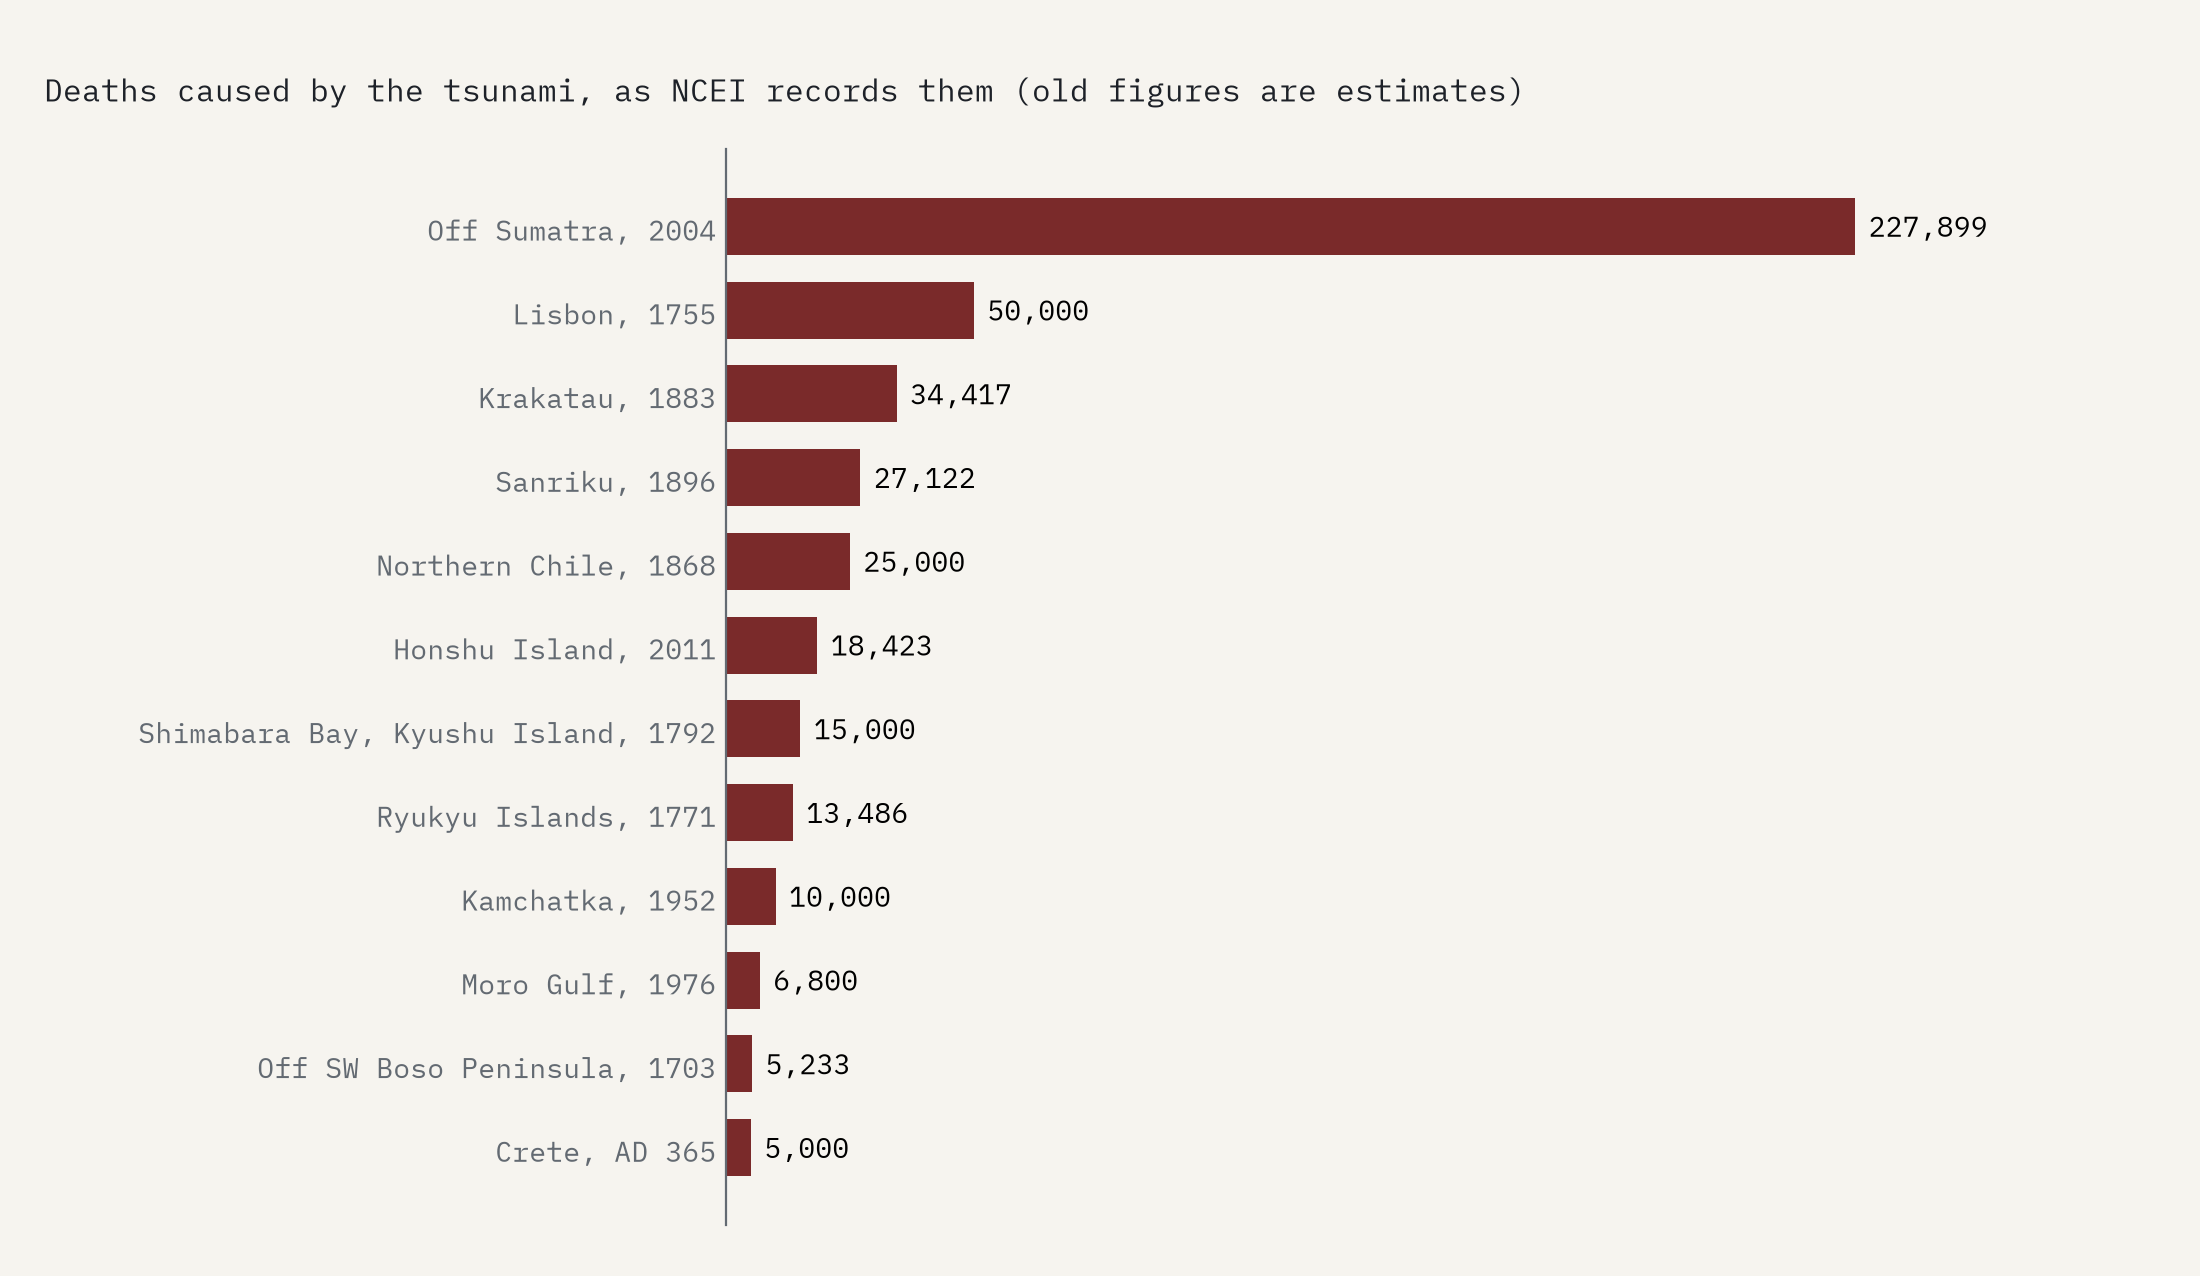
\includegraphics[width=.92\textwidth]{f_deadliest.png}
\caption{The twelve deadliest tsunamis by deaths caused by the tsunami, as NCEI records them.}\label{fig:deadliest}\end{figure}

\subsection{Heights}
NCEI gives a water height for 29,343 places; the median is 2.10 m and 35.9\% are under a metre. 142 tsunamis reached 10 m somewhere, 47 reached 30 m and 9 reached 100 m (Table~\ref{tab:highest}, Figure~\ref{fig:highest}). Every one of the last group involved a landslide or a volcano: the 1958 Lituya Bay rockslide (524.3 m), Tracy Arm in 2025 (481 m), Spirit Lake at Mount St Helens in 1980 (250 m), Vajont in 1963 (235 m) and Dickson Fjord in 2023 (200 m) among them. The highest runup from an earthquake alone is 88 m, at Unga Island, AK in 1788; Tohoku reached 39.3 m and the 2004 tsunami 50.9 m.

\begin{table}[tbp]\centering\footnotesize\caption{The highest runup recorded for each tsunami: the top twelve.}\label{tab:highest}\begin{tabular}{llllr}\toprule Place & Year & Country & Cause & Metres\\\midrule
Lituya Bay, AK & 1958 & United States & Earthquake and landslide & 524.3\\
Tracy Arm, AK & 2025 & United States & Landslide & 481.0\\
Spirit Lake West, WA & 1980 & United States & Volcano & 250.0\\
Casso & 1963 & Italy & Landslide & 235.0\\
Dickson Fjord & 2023 & Greenland & Landslide & 200.0\\
Hoof Hill, Taan Fjord, AK & 2015 & United States & Landslide & 192.9\\
Lituya Bay, AK & 1936 & United States & Landslide & 149.3\\
Lituya Bay, AK & 1853 & United States & Landslide & 120.0\\
Hila, Ambon Island & 1674 & Indonesia & Earthquake and landslide & 100.0\\
Karrat Fjord & 2017 & Greenland & Landslide & 90.0\\
Sado Island & 1741 & Japan & Volcano & 90.0\\
Bureya (81) & 2018 & Russia & Landslide & 90.0\\
\bottomrule\end{tabular}\end{table}

\begin{figure}[tbp]\centering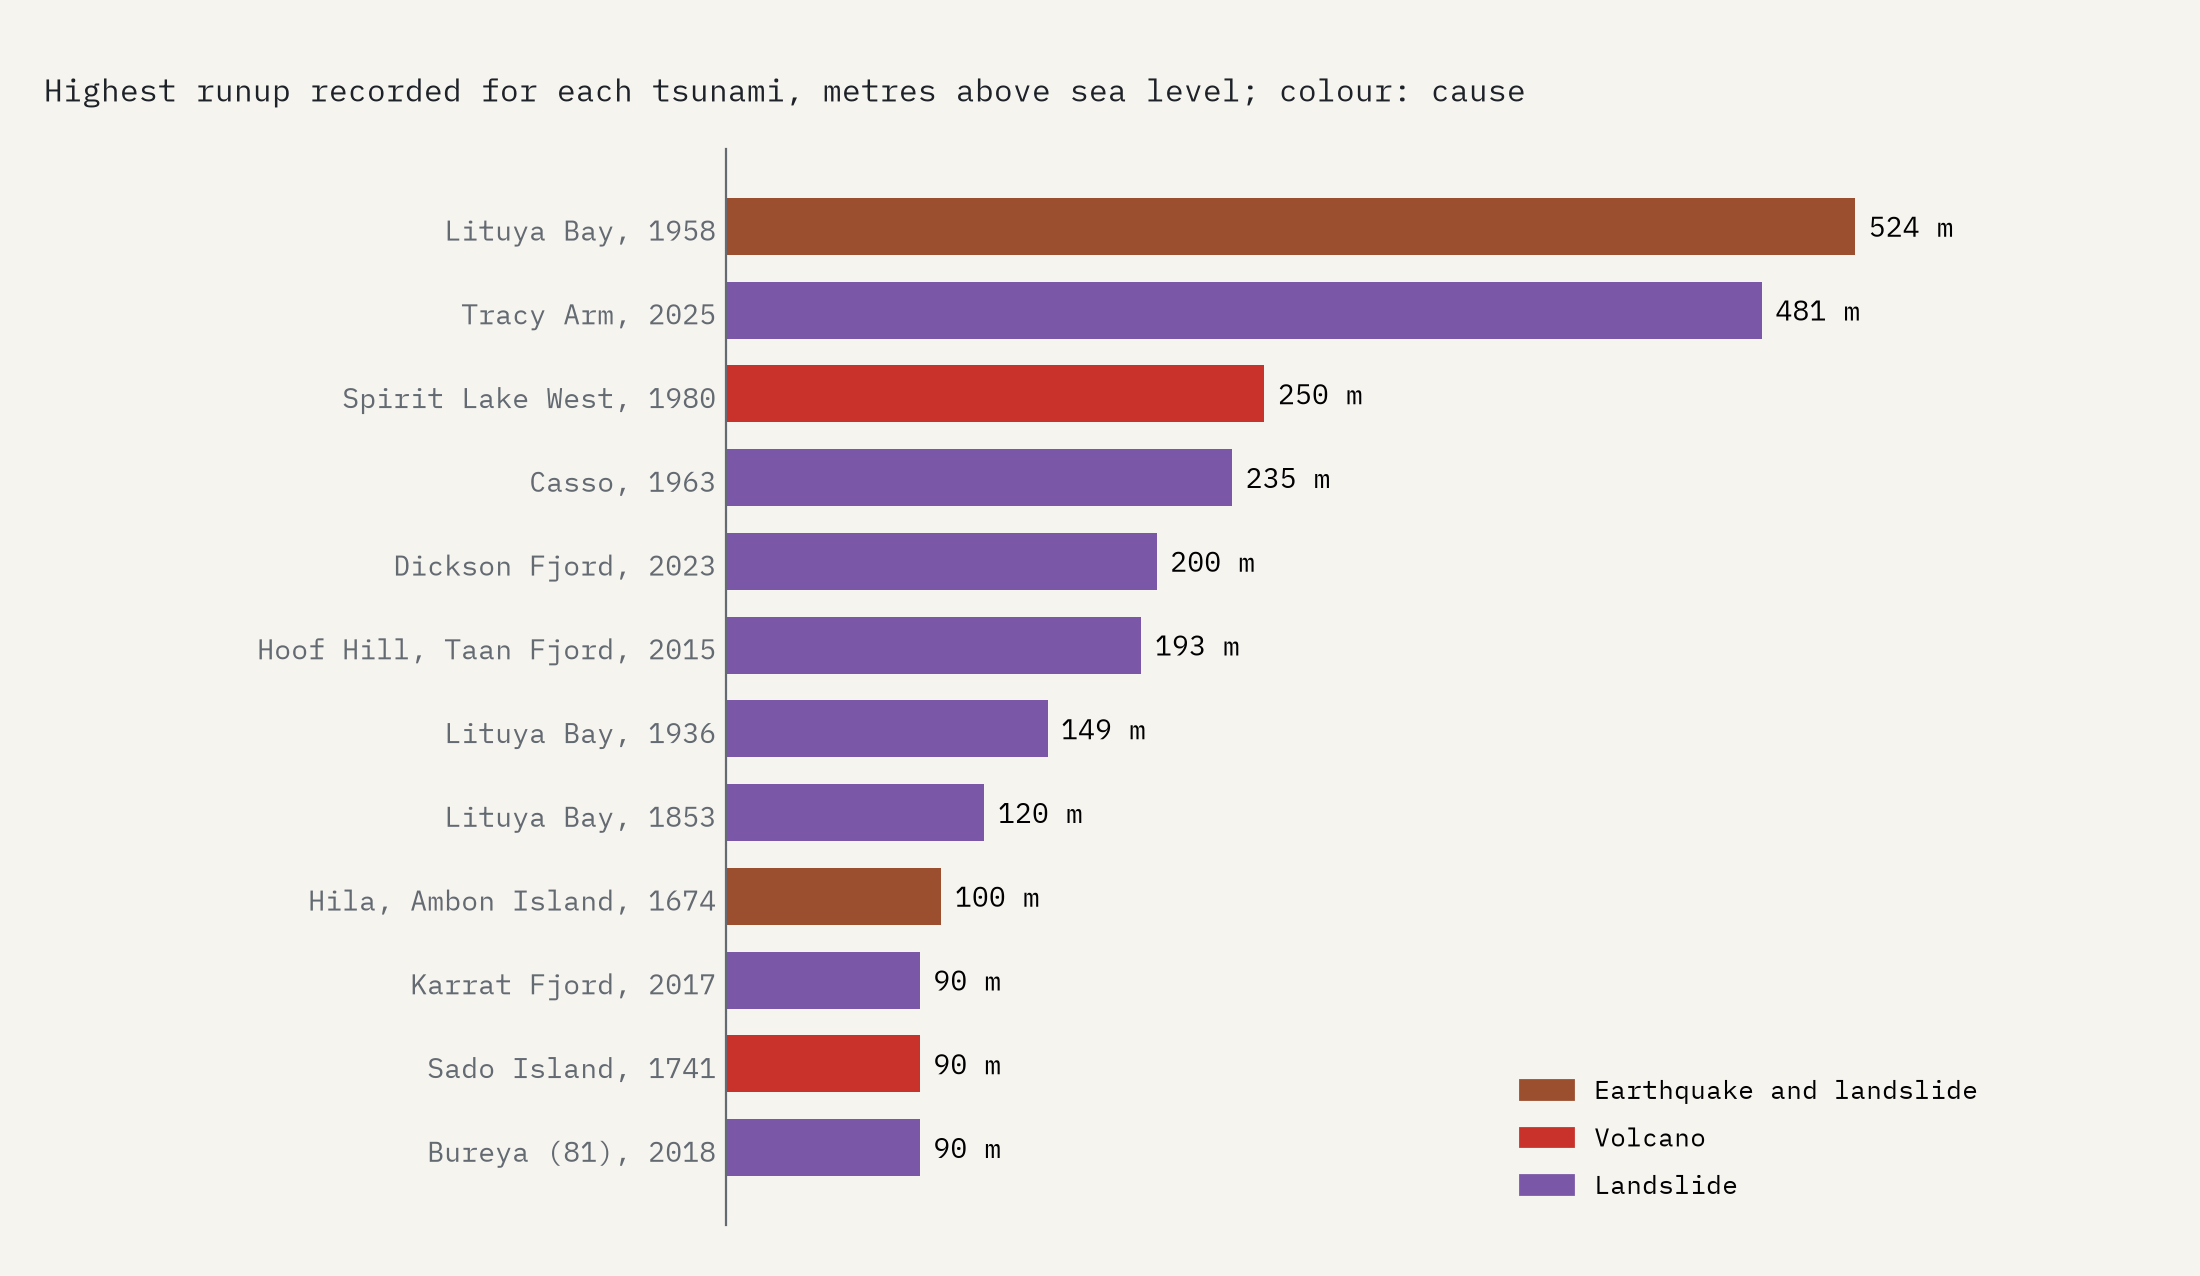
\includegraphics[width=.92\textwidth]{f_highest.png}
\caption{The highest runup recorded for each tsunami: the top twelve, coloured by cause.}\label{fig:highest}\end{figure}

\subsection{Distance and speed}
275 of the 1,060 tsunamis with a measured height and distance (25.9\%) were recorded more than 1,000 km from the source, and 75 more than 10,000 km (Table~\ref{tab:far}). The farthest is 0.20 m at Baltra Island in the Galápagos, 19,266 km from the 2004 source, 29 hours 7 minutes after the earthquake. Most of the rest of the list are Chilean earthquakes recorded in East Asia. Figure~\ref{fig:lines} shows the reach of the 1960 and 2004 tsunamis.

For the 2,403 places more than 1,000 km away with a travel time, the implied speed has a median of 680 km an hour (interquartile range 600 to 730), close to the shallow water wave speed $\sqrt{gh}$ of about 710 km an hour over 4 km of water (Figure~\ref{fig:travel}). Examples: the 1946 Aleutian tsunami reached Hilo, 3,810 km away, in 4.9 hours; the 1960 Chilean tsunami reached Hilo in 14.8 hours and Japan in 22.4; the 2004 tsunami reached Kenya in 8.9 hours, Tanzania in 9.7 and South Africa in 11.1.

The eruptions of Krakatau and Hunga Tonga moved the sea a second way, through their atmospheric pressure waves. NCEI flags 643 such places for Hunga Tonga, in 65 countries as far as Tema, Ghana (18,280 km), and 84 for Krakatau, as far as Colon, Panama. Counting all places, Hunga Tonga reached 67 countries, more than any other event; the 2004 tsunami reached 48.

\begin{table}[tbp]\centering\footnotesize\setlength{\tabcolsep}{4pt}\caption{The farthest place where each tsunami's water was measured (sea waves only, height above zero): the top ten.}\label{tab:far}\begin{tabular}{llrrr}\toprule Tsunami & Farthest place & km & Metres & Hours\\\midrule
Off W. Coast of Sumatra, 2004 & Baltra Island, Ecuador & 19,266 & 0.20 & 29.1\\
Central Chile, 2010 & Lianyungang, China & 18,895 & 0.00 & \\
Northern Chile, 1922 & Takao, Taiwan & 18,828 & 0.00 & 25.8\\
Central Chile, 1985 & Hong Kong, China & 18,671 & 0.10 & \\
Northern Chile, 1995 & Hirara, Japan & 18,440 & 0.10 & \\
Central Chile, 2015 & Yonaguni, Japan & 18,385 & 0.00 & \\
Honshu Island, 2011 & Arraial do Cabo, Brazil & 18,256 & 0.10 & 30.3\\
Southern Chile, 1960 & Hong Kong, China & 18,102 & 0.50 & 27.1\\
Central Chile, 1943 & Nagasaki, Japan & 17,948 & 0.10 & \\
Northern Chile, 1868 & Naha, Ryukyu Islands, Japan & 17,931 & 1.00 & 27.0\\
\bottomrule\end{tabular}\end{table}

\begin{figure}[tbp]\centering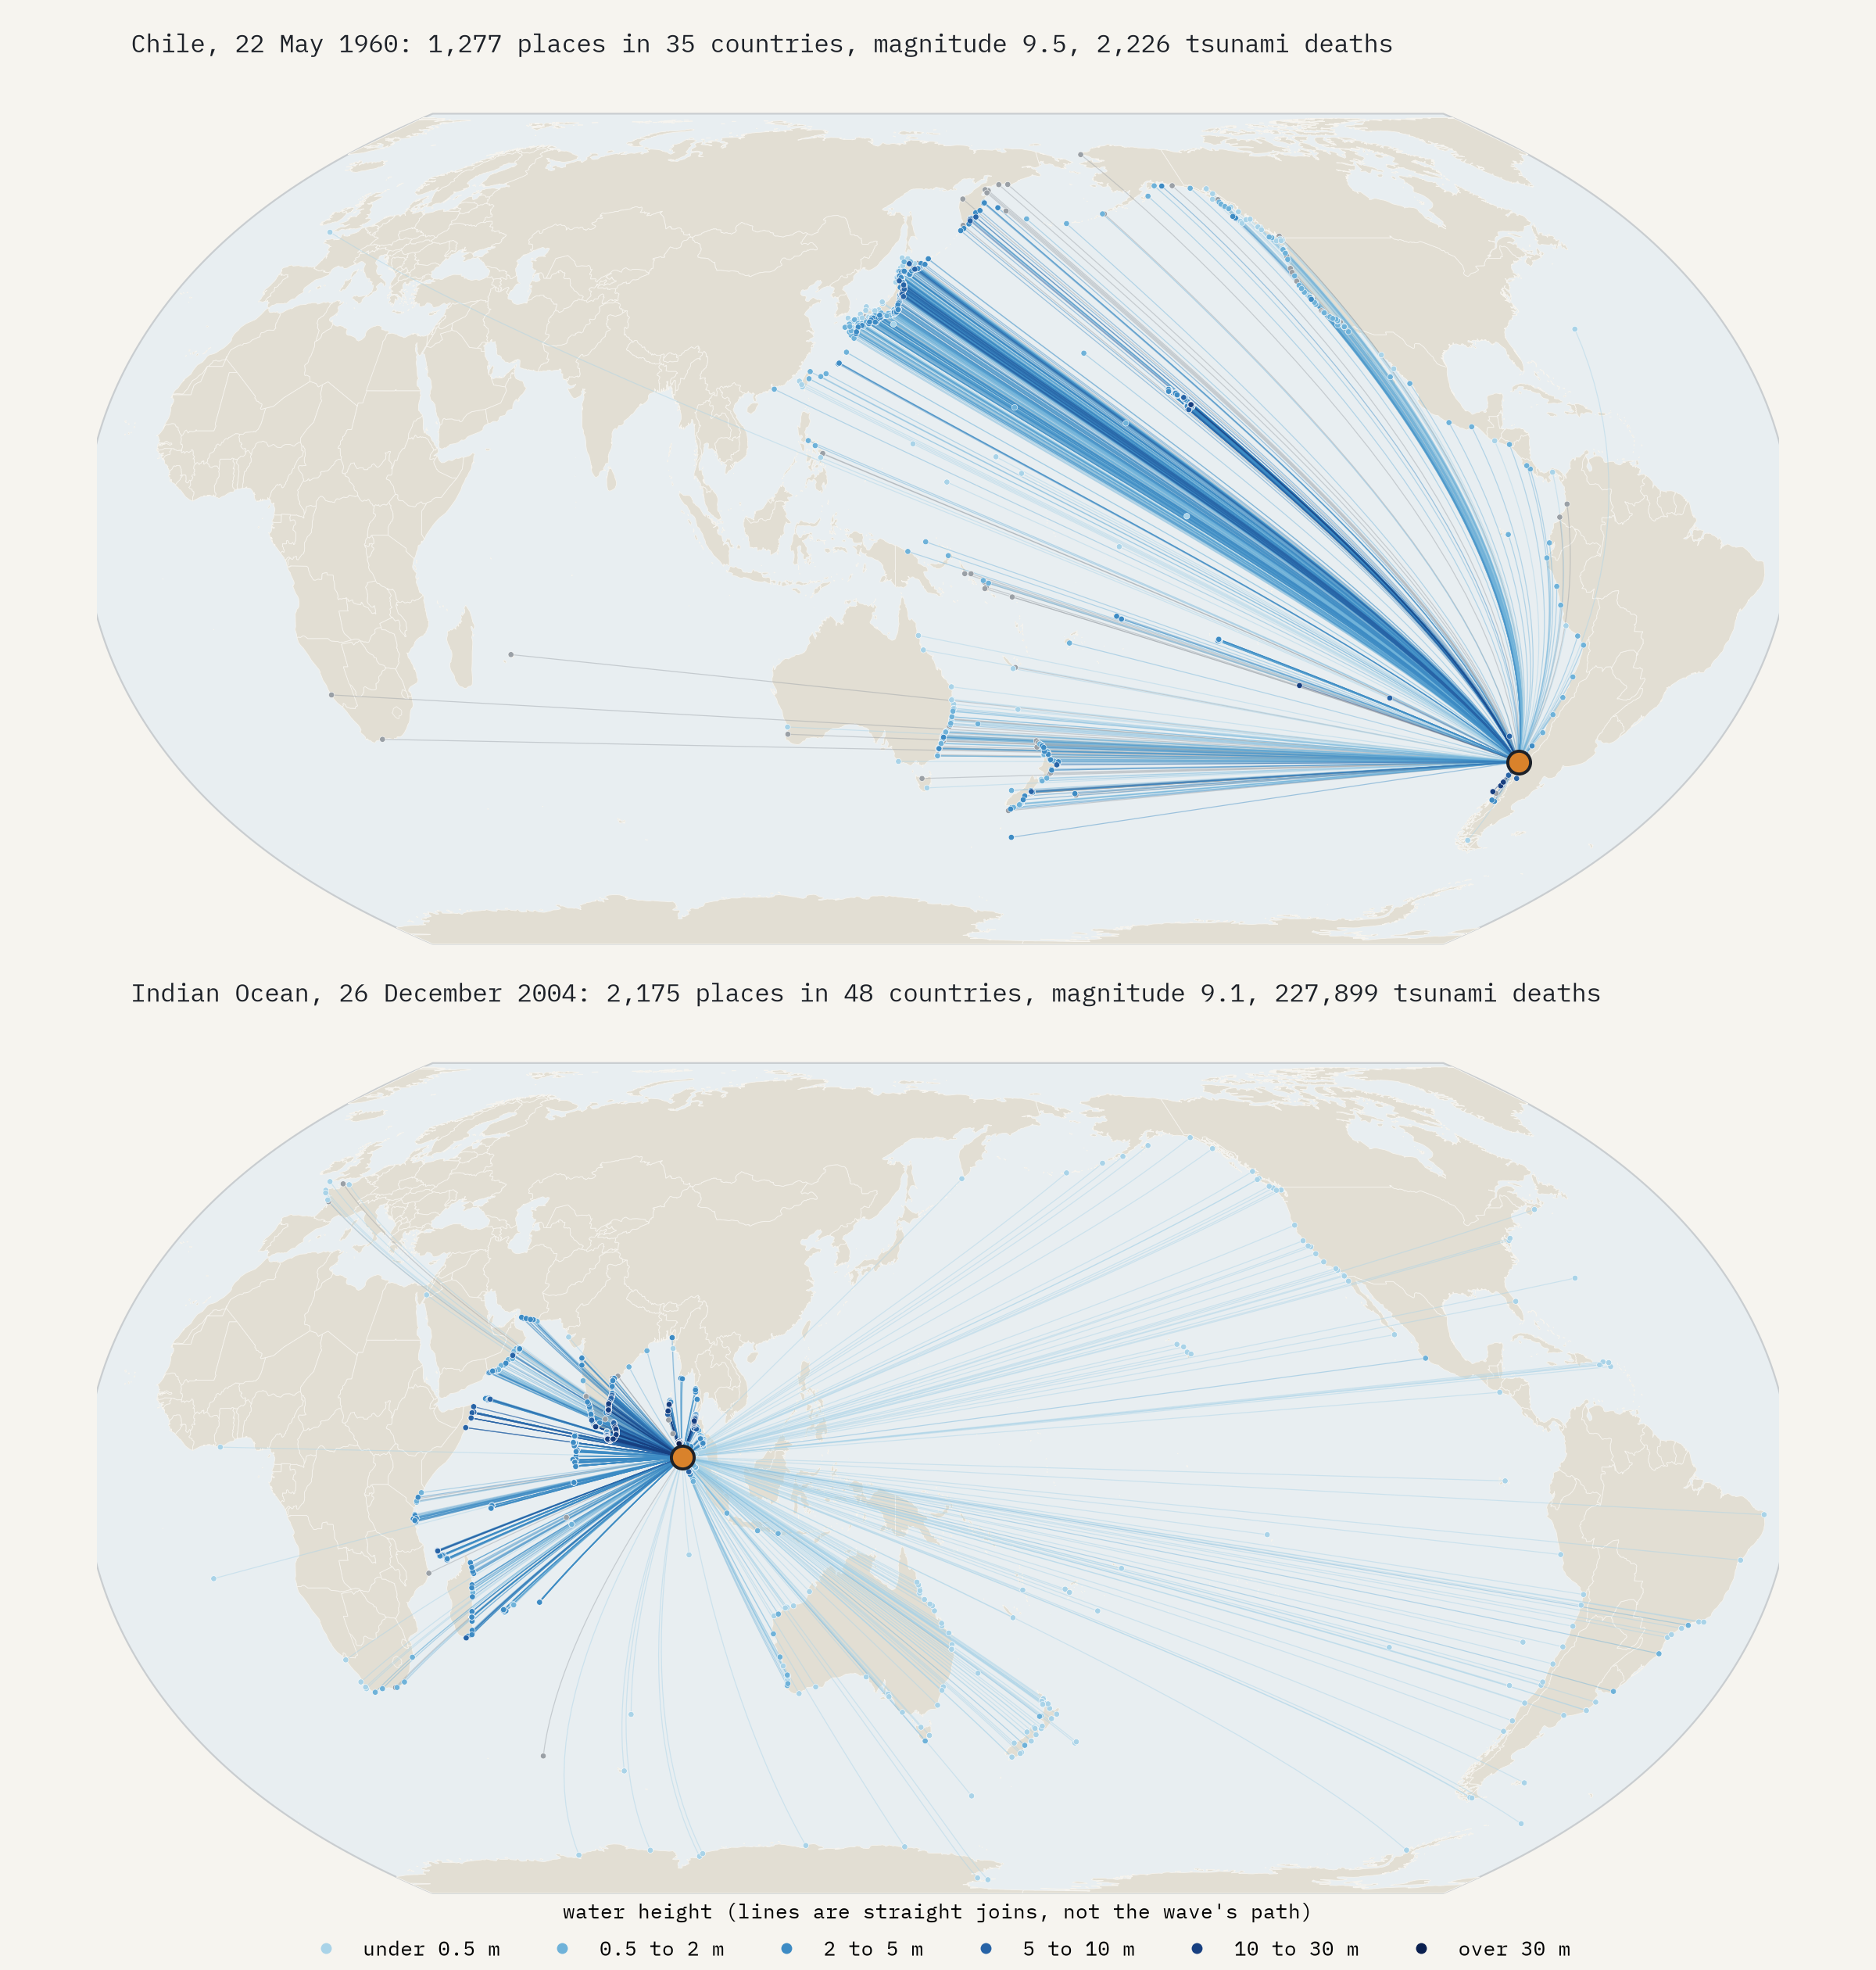
\includegraphics[width=.9\textwidth]{f_lines.png}
\caption{Places where the water of the 1960 Chilean and 2004 Indian Ocean tsunamis was recorded, joined to the source by straight lines and coloured by height.}\label{fig:lines}\end{figure}

\begin{figure}[tbp]\centering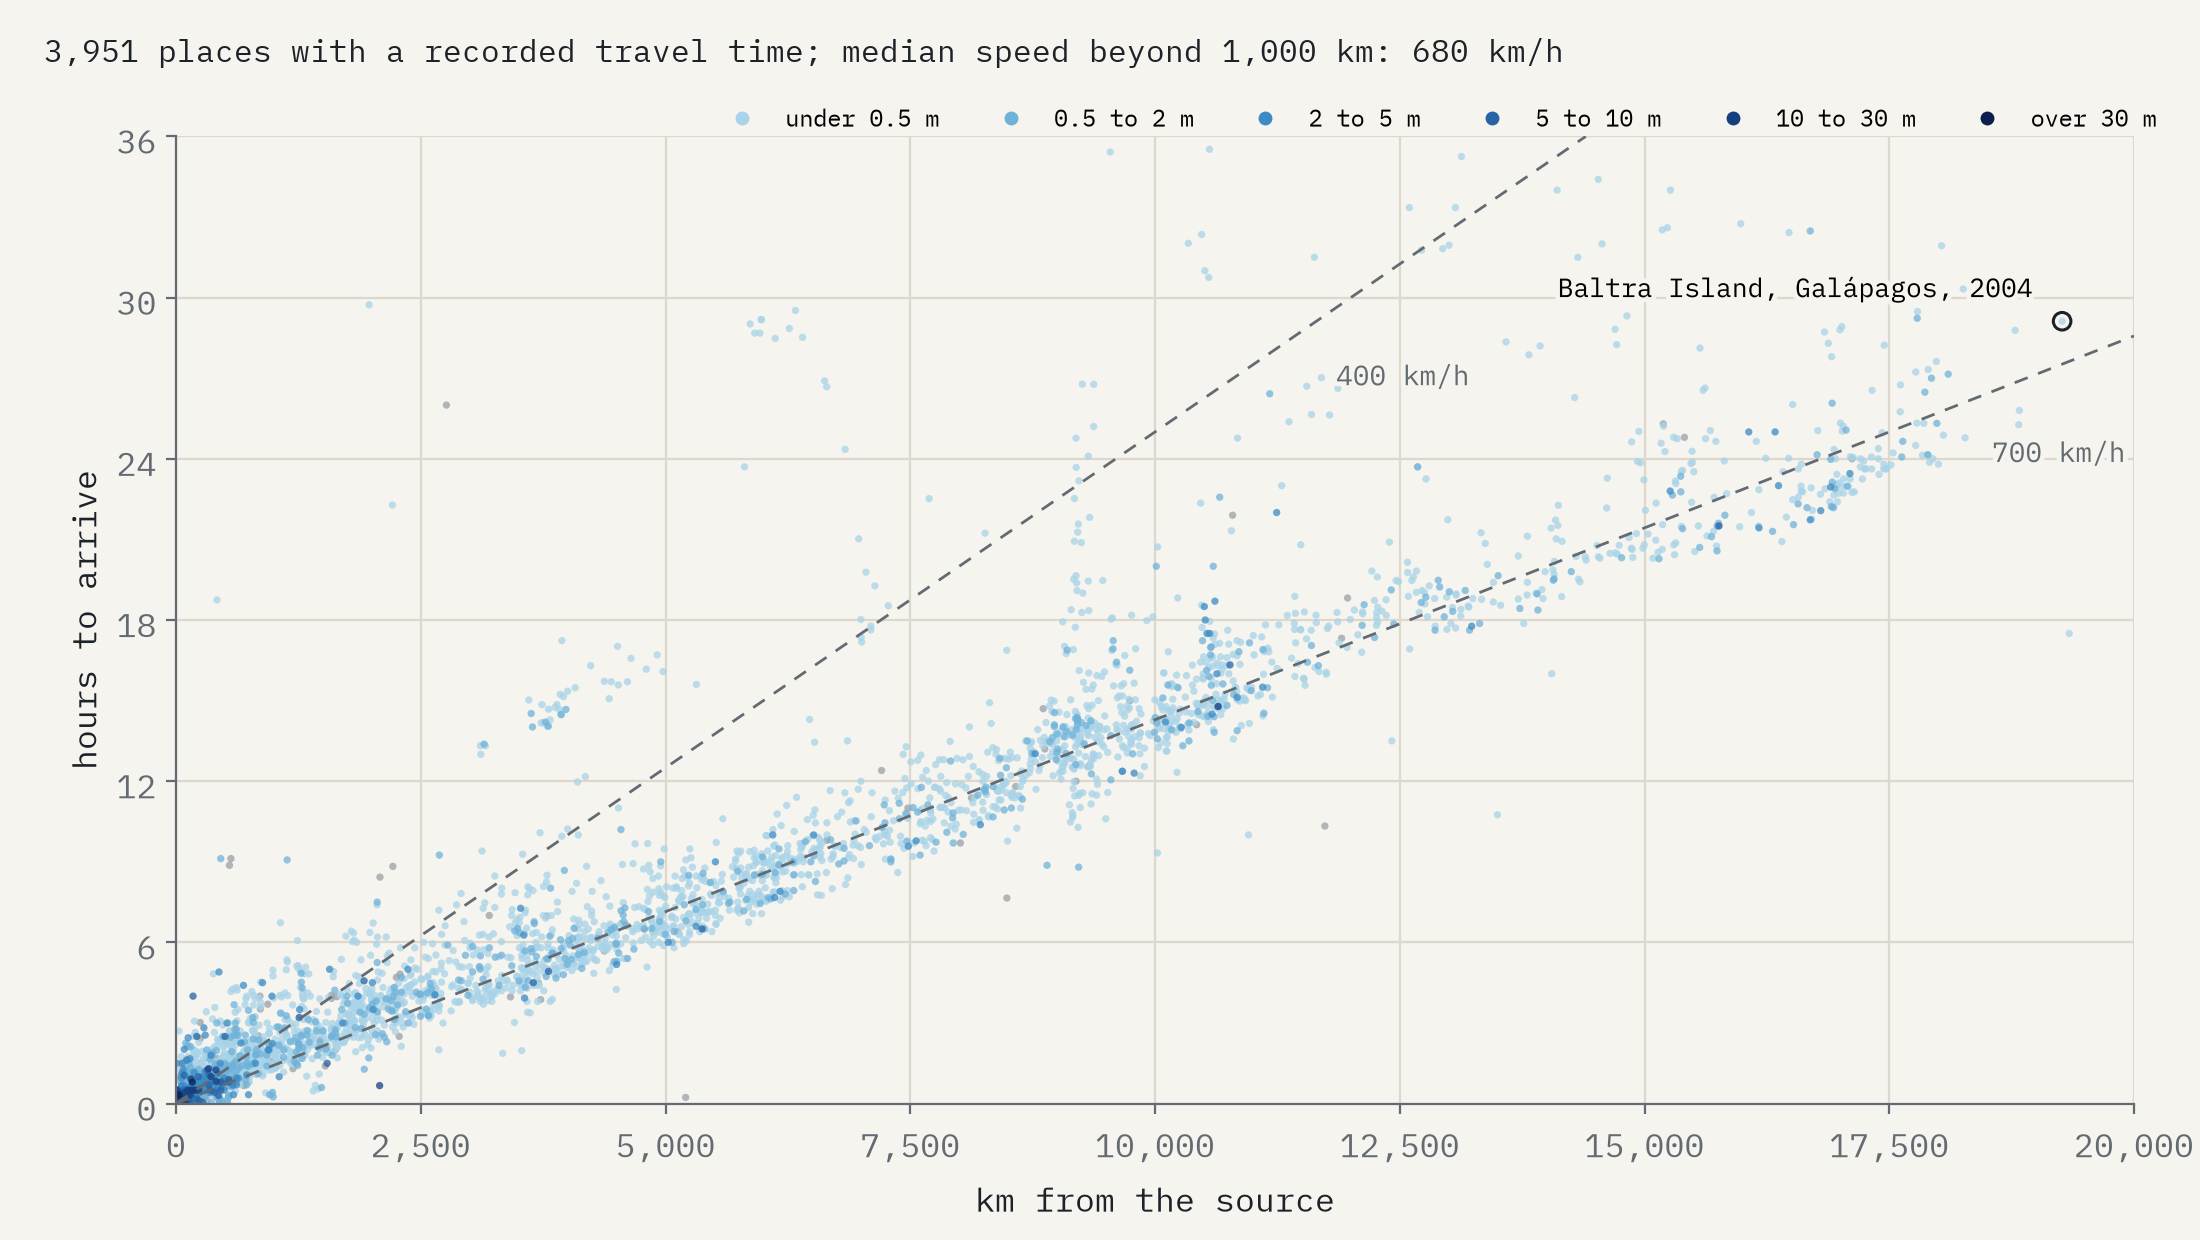
\includegraphics[width=.92\textwidth]{f_travel.png}
\caption{Distance from the source against recorded travel time for every place with both, coloured by water height. Dashed lines: steady speeds of 400 and 700 km an hour.}\label{fig:travel}\end{figure}

\subsection{Through time}
The record is very uneven in time (Figure~\ref{fig:century}). There are 4 tsunamis before AD 1 and 74 before 1500; then 20 in the 1500s, 63 in the 1600s, 88 in the 1700s, 282 in the 1800s and 718 in the 1900s. 69.0\% of the record dates from 1900 or later. This growth is a recording effect: written records spreading around the world's coasts, then tide gauges, seismographs, deep-ocean pressure sensors and systematic surveys, each able to detect smaller waves than before. Meteotsunamis show it most clearly, with 9 recorded before 1950 and 57 since 2000. Even in the instrumental period the decade counts rise, from 63 in 1900 to 1909 to 189 in 2010 to 2019. Since 1950 the database averages 11.5 tsunamis a year, 1.4 of them deadly. None of this is evidence of a trend in tsunami occurrence.

\begin{figure}[tbp]\centering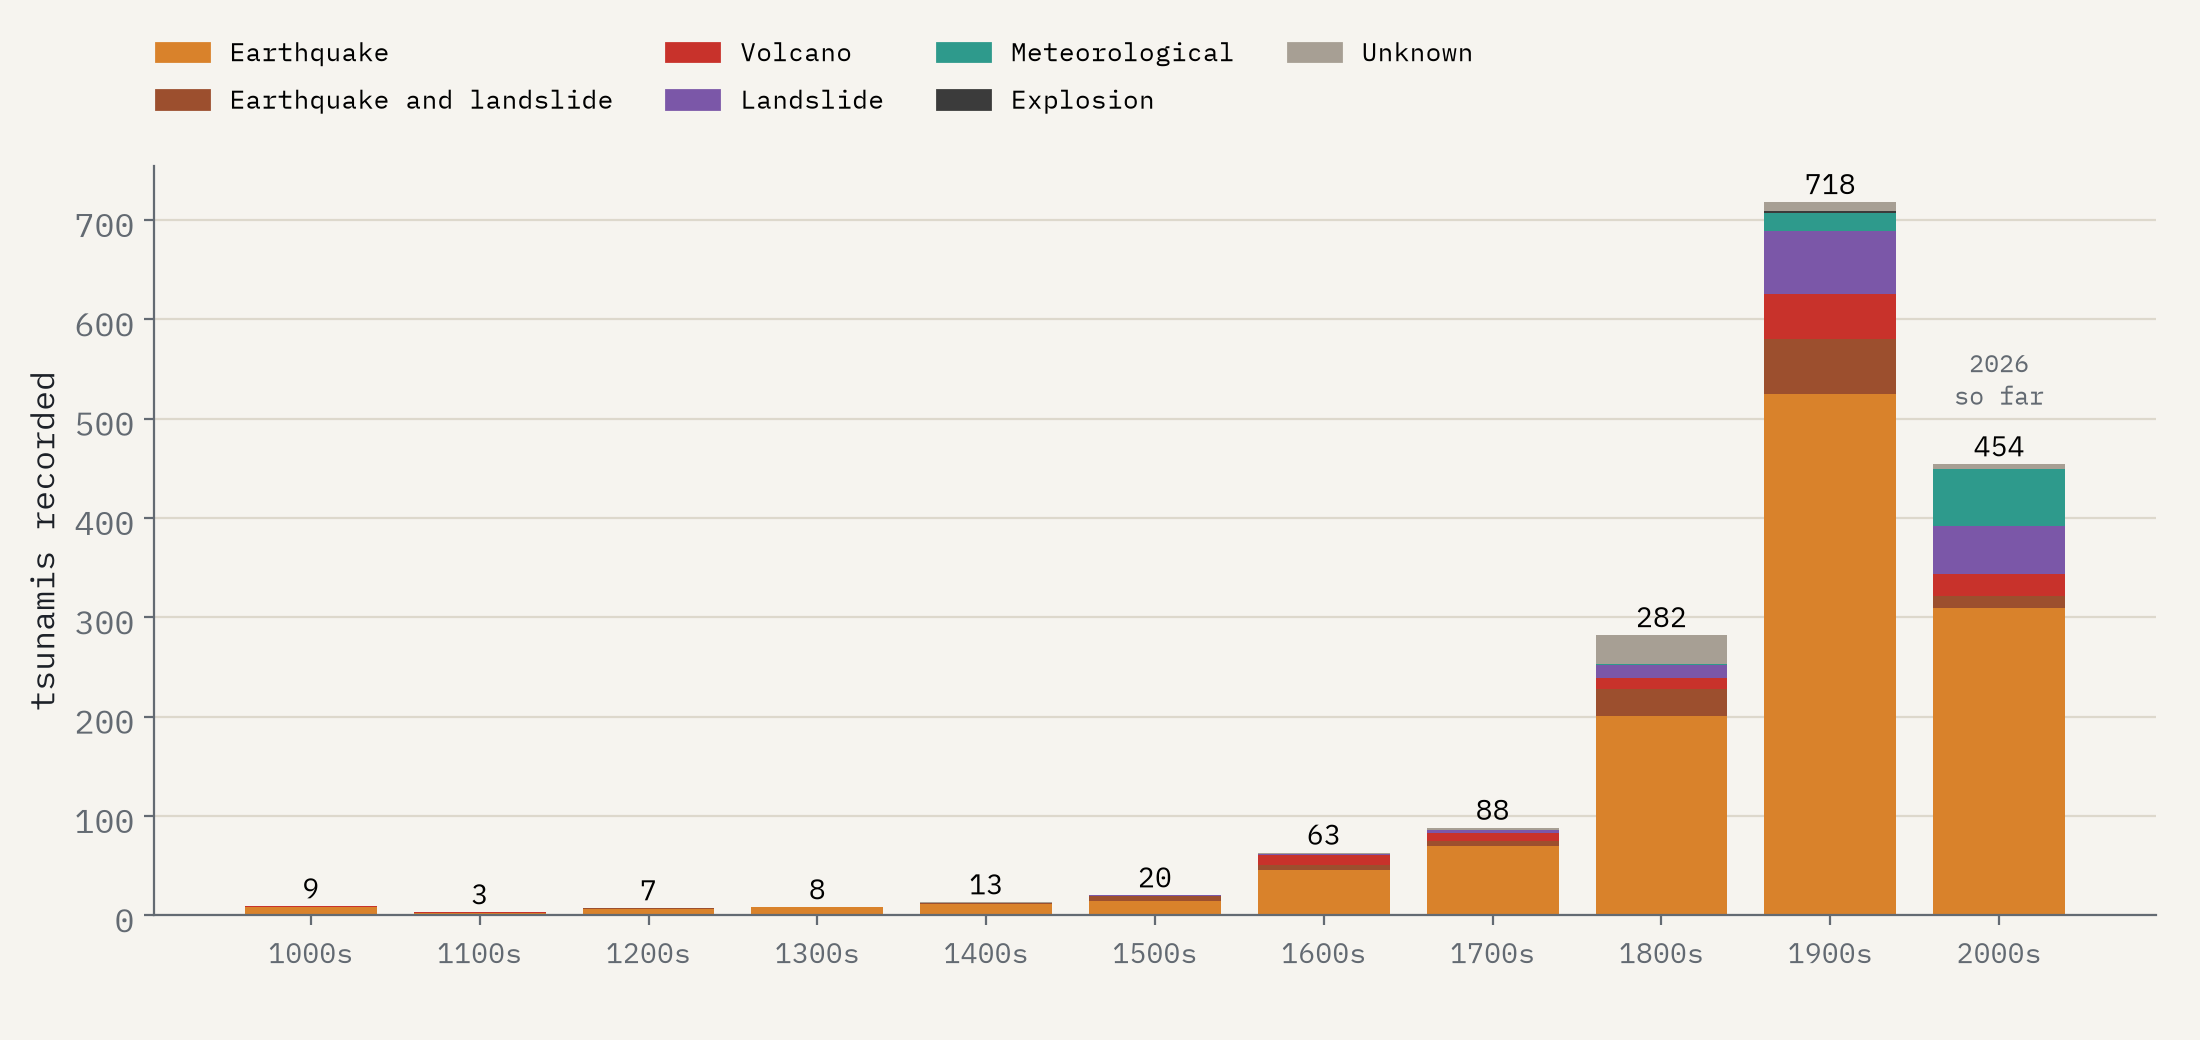
\includegraphics[width=.92\textwidth]{f_century.png}
\caption{Definite and probable tsunamis recorded per century from AD 1000, by cause. The 2000s are partial.}\label{fig:century}\end{figure}

\begin{figure}[tbp]\centering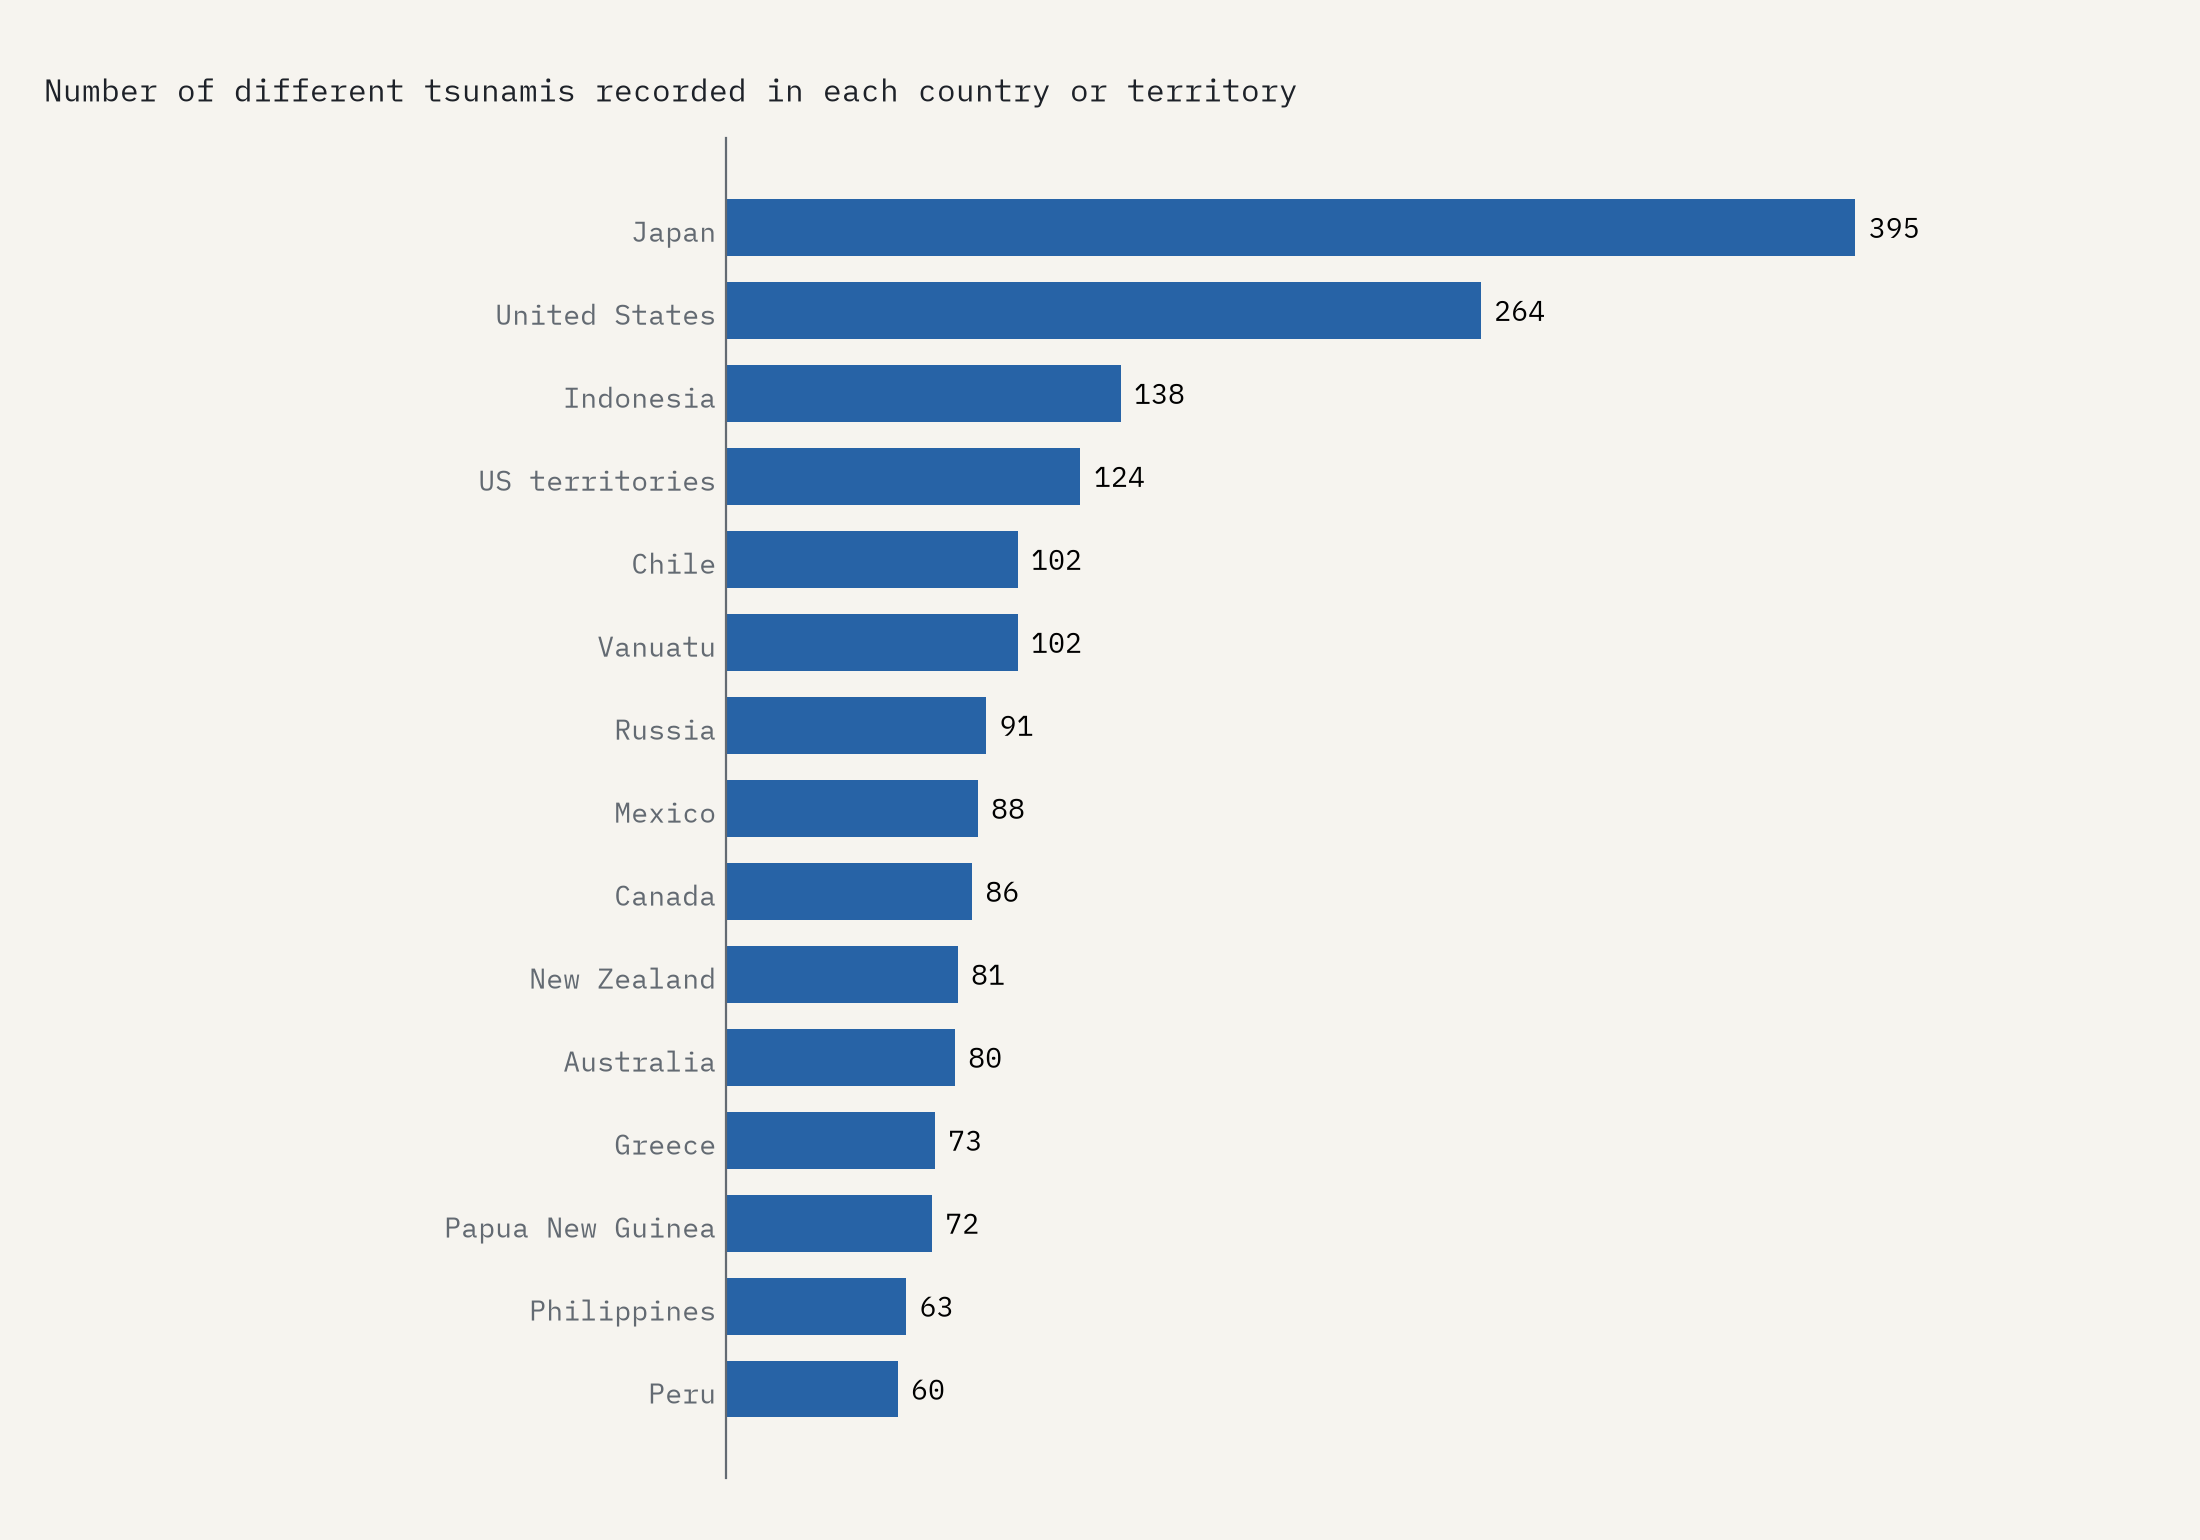
\includegraphics[width=.86\textwidth]{f_countries.png}
\caption{The countries and territories reached by the most tsunamis (number of different tsunamis recorded at one or more places).}\label{fig:countries}\end{figure}

\section{Limitations}
First, the database is a compilation of very different kinds of evidence, and its completeness falls steeply with age; counts over time measure recording effort. Second, validity ratings, causes, dates and positions for old events are NCEI's judgements, which I follow. Third, death tolls for historical events are estimates, sometimes disputed, and many events have none. Fourth, runup records vary from single eyewitness accounts to thousands of survey points for one event, so place counts weight well surveyed events and countries heavily. Fifth, region-based oceans and the Ring of Fire definition are conventions; a different grouping of the Sunda arc changes the Pacific share by a few points. Sixth, 2026 is incomplete.

\section{Conclusion}
Most tsunamis are started by large subduction earthquakes around the Pacific, and at half of the places where their water was recorded it rose 2.1 m or less. The deaths are concentrated in a handful of catastrophes, above all the Indian Ocean tsunami of 2004, which killed more people than every other tsunami of the past century combined in the database. The highest water comes from landslides into confined bays, and the farthest reach from great earthquakes whose waves cross whole oceans at the speed of an airliner, on a timetable that makes warning possible. The growing count of tsunamis is a story about the people and instruments watching the sea.

\section*{Data and code availability}
The interactive map is at \url{https://maps.tristanhotham.com/tsunamis/}. Data and code are at \url{https://github.com/Tristan-Hotham/tsunamis} and archived with this paper at https://doi.org/10.5281/zenodo.23873531. Derived data and text are released under CC BY 4.0 and code under the MIT licence. The NCEI database is a US government work in the public domain; please cite it as below.

\section*{AI statement}
I wrote the text, with drafting and editing assistance from Claude (Anthropic), which also helped prepare the analysis code. I reviewed and checked all text and results.

\begin{thebibliography}{9}
\bibitem[NCEI(2026)]{ncei} National Geophysical Data Center / World Data Service (NGDC/WDS) (2026) NCEI/WDS Global Historical Tsunami Database. NOAA National Centers for Environmental Information. doi:10.7289/V5PN93H7. Fetched 2026 from \url{https://www.ngdc.noaa.gov/hazel/hazard-service/api/v1/}.
\bibitem[Bird(2003)]{bird} Bird, P. (2003) An updated digital model of plate boundaries. \textit{Geochemistry, Geophysics, Geosystems} 4(3), 1027. doi:10.1029/2001GC000252. GeoJSON by H. Ahlenius, \url{https://github.com/fraxen/tectonicplates}, ODC Attribution License.
\bibitem[Natural Earth(2026)]{naturalearth} Natural Earth (2026) Admin 0 countries and populated places, 1:50m and 1:10m. Public domain. \url{https://www.naturalearthdata.com/}
\end{thebibliography}
\end{document}
